\chapter{Data Analysis}
\label{chapter: data analysis}

In this chapter, I will describe the analysis of the data collected in the laser-only experiment conducted in May 2023, with a focus on the spectrometers and their ability to produce spectra capable of high-resolution XAFS. I will start by explaining the processing of the raw images from the cameras into spectra, then I will outline the results to be derived from them. 

I carry out the analysis with a program that I developed in 
\textit{python3} called \textit{AXAWOTLS}, which stands for "Analysis of X-ray Absorption for WDM Observation and Testing of Locally-made Spectrometers". It is capable of reading a 
TIFF image and outputting fully processed spectra, as well as performing further analysis with these spectra. The code is designed from the 
ground up to be applicable to any x-ray spectrometer intended for XAFS and allow "online" data analysis 
during a beamtime, producing results for any given event in less than a few 
minutes. With this processing speed and its ease-of-use, requiring only that the user input parameters, it is my hope that this code lets future researchers involved in WDM 
research with XAFS at PHELIX effectively interpret and act on raw data in a 
beamtime, simplifying the workflow. 

The code consists of two main parts. The first is responsible for producing 
workable spectra from raw TIFF images, while the second encompasses further processing and application of these spectra for 
data analysis.
The general workflow of the code to produce a spectrum is illustrated 
in fig. \ref{fig: analysis overview}. First, horizontal line outs of each 
spectrum in the TIFF image are taken by selecting the corresponding area in the 
image and averaging over the pixels in the vertical direction. This yields the 
counts for each pixel, which are numbered starting from the leftmost edge of 
the image. Next, spectra are flipped depending on the orientation of the camera 
chip and spectrometer channels. The background is subtracted and the 
pixel number is converted to photon energy according to the dispersion of the 
spectrometer. To note is that this dispersion must be first calibrated by a 
previously known emission line, in this work the Al He-$\upalpha$ line.

At this 
point the second part of the code, the data analysis, takes over, further processing the spectra as follows. First, the filters on the spectrometers are corrected out using the transmission 
values from the CXRO database of Berkeley Lab \citep{cxro_database}. Then, the corrected counts $N_{\text{counts}}$ are converted to photon number on detector $N_{\text{det}}$ with the formula
\begin{equation}
N_{\text{det}} = \frac{N_{\text{counts}}\cdot E_{\text{hole}}}{G\cdot E_{\text{ph}}\cdot Qe},
\label{eq: detector correction}
\end{equation}
where the 
gain $G$, energy needed to generate a photoelectron-hole pair $E_{\text{hole}}$, and quantum 
efficiency $Qe$ are all properties of the x-ray camera found in its 
specification sheet. Next, the number of photons emitted by the source per steradian and energy interval $N_{\text{st,eV}}$ is estimated with the equation
\begin{equation}
	N_{\text{st,eV}} = \frac{N_{\text{total}}}{4\pi \Delta E} = \frac{N_{\text{det}}\cdot D}{\Delta x_{\text{pix}}\cdot R_{int}\cdot \Delta E},
	\label{conversion to emitted photons}
\end{equation}
adapted from Döppner \textit{et al.} \citep{doppner2008high}, where $N_{\text{total}}$ represents the total number of photons emitted by 
the source, $D$ 
the distance 
over which the x-rays diverge (for example, the optical path length 
from source 
to detector for flat crystal geometries), $\Delta x_{\text{pix}}$ the 
pixel width in the non-dispersive direction (i.e. the physical length which collects the rays), and $\Delta E$ the energy interval covered by a pixel. Notably, $\Delta E$ is assumed to be constant, as the dispersion of the spectrometers is approximately linear, and the integrated reflectivity $R_{int}$ is taken from the literature, as it is not directly measurable in this experiment. Finally, the spectra can be smoothed through binning over eight pixels, i.e. eight data points.

It is also important to note that the processing is slightly different for the FSSR, where it is summed instead of averaged over the pixel rows of the spectrum to get a horizontal line out. This is due to the imaging properties of the geometry in the non-dispersive direction, as the x-rays only diverge until reaching the crystal, where they are then imaged onto the detector. Accordingly, one must sum the contributions in the non-dispersive direction to accurately represent the signal. As a consequence of the summing, the background is estimated by first averaging to get a horizontal line out, then multiplying by the number of pixel rows summed over for the signal spectrum. As the photons on the camera chip are collected by the entire width of the mica crystal, the diverging distance $D$ and the collecting length $\Delta x_{\text{pix}}$ in formula \ref{conversion to emitted photons} must be adjusted so that $\Delta x_{\text{pix}} \longrightarrow w_{\text{crystal}}$, where $w_{\text{crystal}}$ represents the crystal width in non-dispersive direction, and $D$ becomes the source-crystal distance $a_0$. Otherwise, the spectrum extraction is analogous to the flat crystal geometries.

For finer details of the calculations, please refer to the source code of \textit{AXAWOTLS}, which can be requested by sending me an email at carlosbutler210@gmail.com.

\begin{figure}[H]
	\centering
	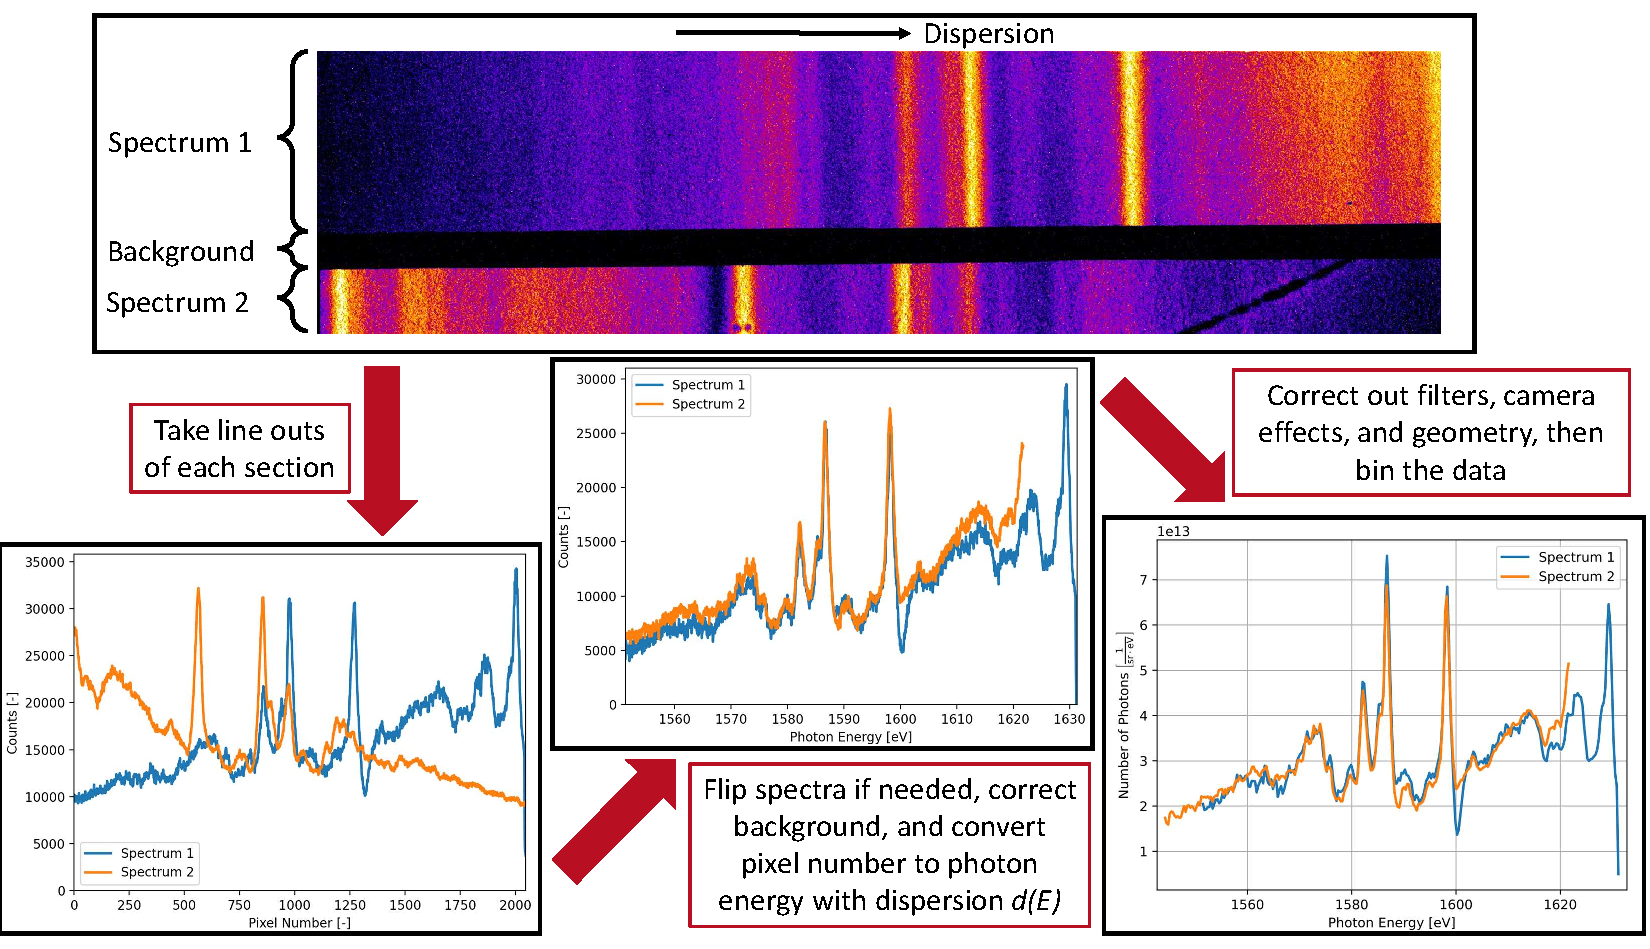
\includegraphics[width=\textwidth]{Data_Analysis/Analysis_overview.pdf}
	\caption{Overview of the data analysis steps from raw TIFF image to fully 
	processed spectrum. Example is of spectra from a Dy plasma ignited with a 
	\SI{57.3}{\joule} laser pulse, recorded with the DUCC. In the raw image, 
	the higher the count, the warmer the color, so yellow represents the maxima 
	and dark purple towards black the minima.}
	\label{fig: analysis overview}
\end{figure}


